\chapter{实验}
\label{cha:exp}
本章介绍验证模型结构所进行的实验。首先,使用Transformer作为基线模型实验了单任务学习下的模型性能,接着使用相同的超参设定实验了~\ref{sec:mtl_tf}~节介绍的四种多任务Transformer的性能。具体地,在第~\ref{sec:task}~节介绍实验任务,在第~\ref{sec:ds}~节介绍数据集相关信息,在第~\ref{sec:results}~节介绍实验结果。最后,~\ref{sec:analysis}~节给出了实验分析。

\section{任务描述}
\label{sec:task}
我们在\emph{文本分类}(Text Classification)这一经典NLP任务上进行实验。事实上,很多NLP问题都可以归为文本分类的范畴,例如情感分析(Sentiment Analysis, SA)、自然语言推理(Natural Language Inference, NLI)等。在目前被广泛使用的多任务基准数据集GLUE\cite{DBLP:conf/emnlp/WangSMHLB18}中,所有任务都可以被归为文本分类任务。

文本分类即将一段归到某个特定的预先定义的类别。待分类的文本通常是一个句子(如情感分析)或一个句子对(如自然语言推理)。需要注意的是,这里的一个句子并不一定是常规意义上以一个句号为结束标识符的一句话,也有可能包含多句话。文本分类任务在现实生活中也有着广泛的应用,如自动分析产品评价、微博情感分析、文档标签分类等等。

文本分类任务需要模型能够抽取出易于分类的句子表示,然而不同领域中通常需要关注不同的特征,例如在食物类的评论文本中模型应当更加关注“好吃”、“美味”等词,而在电影评论文本中应当更加关注“好看”、“烂片”等词语。同时,不同领域的文本分类任务常常也需要某些通用的特征,如“很棒”、“优秀”等词在所有与主观倾向有关的分类任务中都是应当被关注的。而事实上,在某个特定的领域内,文本数据量常常是有限的,这种情况下单任务学习通常难以取得很好的效果,可以通过多任务学习来利用其他领域的相关知识帮助分类。

\section{数据集}
\label{sec:ds}
我们的基线单任务模型以及多任务模型在16个文本分类数据集上进行了对比实验,其中的前14个数据集来自亚马逊的产品评论\footnote{\url{https://www.cs.jhu.edu/˜mdredze/datasets/ sentiment/}},但是来自各自不同的领域,如图书、电子、光盘等。该部分数据由Blitzer等人\cite{DBLP:conf/acl/BlitzerDP07}收集而成,其余两个数据集IMDB\cite{DBLP:conf/acl/MaasDPHNP11}和MR\cite{DBLP:conf/acl/PangL05}则来自电影评论。每个数据集包含约2000个样本,其中70\%划分为训练集,10\%划分为验证集,20\%划分为测试集。数据集的具体统计信息见表~\ref{tb:dataset}。

\begin{table}[htb]
	\centering
	\caption{数据集统计数据}
	\begin{tabular}{ccccccc}
		\toprule[2pt]
		数据集&训练集大小&验证集大小&测试集大小&类别数&平均长度&词表大小\\
		\midrule[1pt]
		Books& 1400& 200& 400& 2& 159& 19K\\
		Elec& 1398& 200& 400& 2& 101& 11K\\
		DVD& 1400& 200& 400& 2& 173& 20K\\
		Kitchen& 1400& 200& 400& 2& 89& 9K\\
		Apparel& 1400& 200& 400& 2& 57& 7K\\
		Camera& 1397& 200& 400& 2& 130& 9K\\
		Health& 1400& 200& 400& 2& 81& 9K\\
		Music& 1400& 200& 400& 2& 136& 17K\\
		Toys& 1400& 200& 400& 2& 90& 10K\\
		Video& 1400& 200& 400& 2& 156& 17K\\
		Baby& 1300& 200& 400& 2& 104& 8K\\
		Mag& 1370& 200& 400& 2& 117& 11K\\
		Soft& 1315& 200& 400& 2& 129& 11K\\
		Sports& 1400& 200& 400& 2& 94& 10K\\
		IMDB& 1400& 200& 400& 2& 269& 25K\\
		MR& 1400& 200& 400& 2& 21& 7K\\
		\bottomrule[2pt]
	\end{tabular}
	\label{tb:dataset}
\end{table}

\section{实验结果}
\label{sec:results}
实验结果如表~\ref{tb:results}~所示,我们的四个多任务模型在十六个文本分类任务上均超过了单任务训练的表现,验证了多任务学习在Transformer上的有效性。其中,L-I结构在四种多任务架构中表现最好,S-P结构表现最差。L-I结构和L-E结构取得的较好结果表明,在每一层都形成任务特定表示的做法相比在网络的顶层获取特征更为合理。同时,注意到S-C结构也能达到较好的准确率,这也肯定了之前被广泛使用的硬共享模式的效果,但随着任务之间差异性的增大,我们有理由认为L-I和L-E的共享架构相比传统架构将表现出更大的优越性。

\begin{table}[htb]
	\centering
	\caption{模型在测试集上的分类准确率}
	\begin{tabular}{c|cccccc}
		\toprule[2pt]
		\multirow{2}*{数据集}&\multirow{2}*{单任务}&\multicolumn{4}{c}{多任务}\\
		\cline{3-6}
		&&S-P结构& S-C结构& L-I结构& L-E结构\\
		\midrule[1pt]
		Books& 83.50& 82.50& 84.00& 85.00& 84.50\\
		Elec& 79.50& 82.50& 83.50& 84.75& 85.75\\
		DVD& 82.75& 84.50& 85.50& 85.75& 85.75\\
		Kitchen& 79.50& 83.50& 85.00& 89.00& 87.75\\
		Apparel& 82.75& 85.50& 86.75& 86.00& 85.75\\
		Camera& 81.75& 84.25& 85.00& 87.00& 89.00\\
		Health& 86.00 & 85.50& 87.50& 88.00& 86.75\\
		Music& 76.50& 83.00& 83.00& 82.75& 81.50\\
		Toys& 80.00& 84.75& 86.25& 88.25& 86.50\\
		Video& 84.75& 81.25& 85.50& 86.50& 84.25\\
		Baby& 81.00 &87.75& 85.50& 87.25& 87.50\\
		Mag& 89.00& 85.00& 91.00& 89.75& 89.25\\
		Soft& 86.50& 86.00& 88.75& 86.50& 87.75\\
		Sports& 80.25& 84.25& 83.75& 86.00& 85.50\\
		IMDB& 80.75& 84.75& 85.00& 84.50& 84.50\\
		MR& 75.25& 76.00& 75.75& 78.00& 76.50\\
		\rowcolor{lightgray}
		AVG.& 81.86& 83.81& 85.11& \textbf{85.94}& 85.53\\
		\bottomrule[2pt]
	\end{tabular}
	\label{tb:results}
\end{table}

在实践中,神经网络的层数通常是一个比较重要的超参数,模型性能有时会由于层数的不同而产生较大差异。之前的实验中使用的模型均为4层Transformer,为探究多任务Transformer结构对网络层数的敏感性,我们实验了四种结构在不同层数下的平均分类准确率,结果如图~\ref{fig:layer_dis}~所示。

可见,在各个层数设定中,逐层共享结构(L-I结构和L-E结构)均优于传统的硬共享结构(S-P结构和S-C结构),且L-I结构在三种设定中都取得了最优准确率,这一实验结果证明了模型的鲁棒性。

\begin{figure}[htb]
\centering
\begin{tikzpicture}
\begin{axis}[
	xlabel={层数},
	ylabel={准确率},
	legend style={
		cells={anchor=east},
		legend pos=outer north east,
	}
]

\addplot coordinates{
	(2, 0.8547)
	(4, 0.8594)
	(6, 0.8523)
};

\addplot coordinates{
	(2, 0.8539)
	(4, 0.8553)
	(6, 0.8500)
};

\addplot [mark=x]coordinates {
	(2, 0.8451)
	(4, 0.8381)
	(6, 0.8167)
};

\addplot coordinates{
	(2, 0.8484)
	(4, 0.8511)
	(6, 0.8478)
};
\legend{L-I结构,L-E结构,S-P结构,S-C结构}
\end{axis}
\end{tikzpicture}
\caption{网络层数对测试集准确率的影响}
\label{fig:layer_dis}
\end{figure}

\section{实验分析}
\label{sec:analysis}

\begin{figure}[htb]
\centering
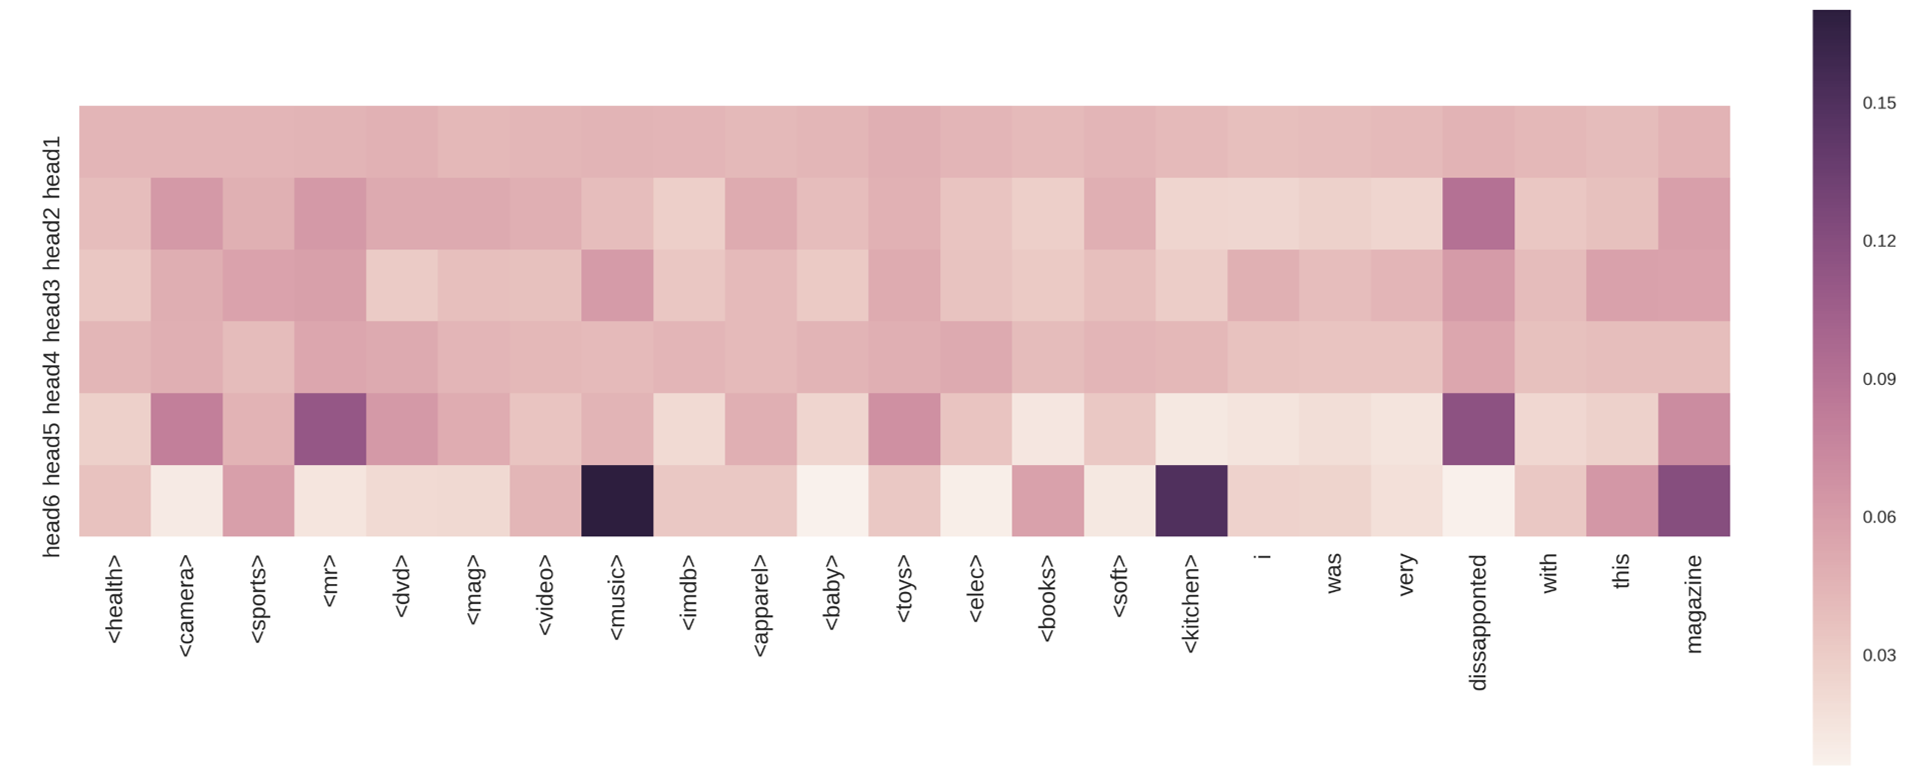
\includegraphics[scale=0.4]{L-E-attn.png}
\caption{L-E结构注意力可视化}
\label{fig:l-e-attn}
\end{figure}